\chapter{Study of functional programming abstractions for concurrency and asynchronicity}
\label{chap:study}

The architecture of the platform is heavily based on functional programming concepts to handle concurrency and
asynchronicity in an effective and composable way. The following section describes and compares these abstractions.


\section{Monadic Futures}

\subsection{The problems of blocking IO with threads}

To handle concurrency and IO, traditional languages use native threads and blocking IO. A thread is a unit of execution that is has its own stack
on the underlining OS, and concurrency is achieved by switching threads on the machine cores. For example, with the blocking IO model,
a thread that is waiting for IO is preempted by the OS. Traditionally threads has a high resource cost, both fixed cost (the default stack size for a thread is 
1 MB on a 64 bit JVM), high context switching cost and high creation time. In case of Web-oriented application, a new thread is generally spawn for each new client,
and if the Web application needs to call several backend services (that is usually the case in modern Service Oriented Architecture), 
this thread will be blocked, doing nothing but using stack space and causing context switching.
Such a model has been proved to be inefficient for a large number of concurrent clients for Web applications that calls various backend services
and/or perform stream-oriented connections as highlighted by James Roper \footfullcite{bib:asyncio}. This is ever more
important when backend services can occasionally be slow / fail. In case of a blocking IO model, clients' threads that requests
this failed service will wait for this service (before a timeout), causing a very high number of threads in the server. As James Roper
stated, this high number of threads prevents the other requests (calling another non-failed service) to be performed efficiently,
because the server spends a lots of its time doing context switching between blocked threads that are doing nothing. This is ever worst if
you have a maximum number of threads allowed in the server (that is usually the case in cloud platforms): new clients can not connect at all
to your server because there is no thread to allow to them. Non-blocking IO servers are also known as evented servers.
Mark McGranaghan highlights this in his article about Threaded vs Evented Servers \footfullcite{bib:threadevent}. If we define \verb|c| the CPU time
that each request takes and \verb|w| the total time of the request including waiting time calling external services, an evented server
performs way better than a threaded server when the ratio \verb|w/c| is high (so when most time of a request is spent waiting for
external services).

\subsection{The problems of asynchronous non-blocking IO with callbacks}
In order to avoid the problems caused by blocking IO, one can use a non-blocking IO model: when a thread is doing an IO operation, it doesn't wait
until the IO is finished but rather provide a mechanism to notify the caller when the IO is finished. Meanwhile, the thread can be used for other tasks, like
serving other web clients. 

The problem is that this kind of asynchronous non-blocking programming can easily lead to hard code maintenance if no proper abstraction is used. The common way
of many languages to deal with asynchronicity is to provide a callback mechanism (Javascript may be the language that uses them the most). A callback is
way to perform an asynchronous operation by providing a function as a parameter of the function that do the asynchronous operation. The parameter function
will be \textit{call back} when the asynchronous operation is finished. An example of a GET HTTP request to a web service in Javascript is shown in Listing 
\ref{lst:jscb}.

\begin{listing}[h]
\begin{minted}[fontsize=\codesize, frame=lines, framesep=2mm]{javascript}
performHttpGet("http://www.example.com", function(error, response) {
  if (!error) {
    console.log("Response status: " + response.status)
  }
});
\end{minted}
\caption{A callback in Javascript}
\label{lst:jscb}
\end{listing}

Here \verb|function(error, response) {...}| is the user-defined function that is call back when the asynchronous GET request
returned. We see that callbacks are only about side-effects: no value is returned by the \verb|performHttpGet| function.
This causes a serious lack of composability, popularly known as "callback hell". Listing \ref{lst:jspd} shows how to perform several asynchronous operations
sequentially.

\begin{listing}[h]
\begin{minted}[fontsize=\codesize, frame=lines, framesep=2mm]{javascript}
action1(function(error, response1) {
  if (!error) {
    action2(function(error, response2) {
      if (!error) {
        action3(function(error, response3) {
          if (!error) {
            action4(function(error, response4) {
              // do a side-effect with response4       
            });
          }
        });
      }
    });
  }
});
\end{minted}
\caption{The "pyramid of doom" in Javascript}
\label{lst:jspd}
\end{listing}

Such call is called "pyramid of doom" because the code invariably shifts to the right, and the intermediate steps can not be reused to compose
them later with other operations. 

Moreover, doing concurrent operations with the callback model is not easy also. We want here to perform 2 asynchronous operations in parallel,
and do something with the result (composed of the result of the 2 operations). Listing \ref{lst:jsparr} shows how to do such in standard Javascript.

\begin{listing}[h]
\begin{minted}[fontsize=\codesize, frame=lines, framesep=2mm]{javascript}
  var results = [];

  function doSomethingWithResults(results) {
    // final callback
  }

  action1(function(error, response) {
      results.push(response);
      if (results.length == 2) {
        doSomethingWithResults(results)
      }
    }
  });

  action2(function(error, response) {
    results.push(response);
    if (results.length == 2) {
      doSomethingWithResults(results)
    }
  });
\end{minted}
\caption{Performing two asynchronous operations concurrently in Javascript}
\label{lst:jsparr}
\end{listing}

The fact that the callback model is based on a closures that performs side-effect prevents easy composability. What I mean by composabilty
is the fact of defining independently various asynchronous operations, and then compose them (sequentially, in parallel) to obtain a composed result
of these actions. Moreover, error handling must be done manually for each asynchronous operation. Monadic futures are an abstraction coming from
functional programming that solves these problems.


\subsection{Monadic futures for composable asynchronous non-blocking programming}

A Future is a monadic abstraction that stands for a value that may be available in the future. Using Scala's notation, a future is a type that is 
parametrized by the type of the value that will eventually be available. For example, \verb|Future[Int]| is a type that represents an eventual integer.
With futures, asynchronous functions return a \verb|Future[ResponseType]| instead of taking a callback function as a parameter. Listing \ref{lst:futures}
shows simple future creations.

\begin{listing}[h]
\begin{minted}[fontsize=\codesize, frame=lines, framesep=2mm]{scala}
val futureResponse: Future[HttpResponse] = performHttpGet("http://www.example.com")
val futureComputation: Future[Int] = future {
  // do long computation
}
\end{minted}
\caption{Futures in Scala}
\label{lst:futures}
\end{listing}

We see in Listing \ref{lst:futures} that futures can be used for non-blocking IO, but also as an abstraction for concurrency. In the example, the main thread
executing the code does not block on both methods. The "long computation" will be done in another thread as it is encapsulated by a \verb|future {}|.

Behind the scene, futures are multiplexed into a thread pool named a ExecutionContext in Scala. ExecutionContexts can be passed to methods that returned a future.
This allows to decouple the \textit{concurrency semantic} (which tasks should be run concurrently) from the \textit{concurrency implementation} (an ExecutionContext
can for example limit the number of threads it can use, etc.). Twitter's engineer and researcher Marius Eriksen highlights this idea in his 
"Your Server as a Function" paper \footfullcite{bib:serverfunc} where he states that futures are a declarative data-oriented way of doing asynchronous programming.

Moreover, as Marius Eriksen highlights in his article "Future aren't ersatz threads" \footfullcite{bib:futurenotthreads}, Futures "model the real world truthfully": 
a Future[T] can either result in a success with a value of type T, or with an error (Exception), which is inherently the case with IO operations.
\\

The term \textit{monadic} comes from Monads, a key abstraction in typed functional programming coming from the Haskell world. Thoroughly defining what a monad
is out of the scope of this thesis, but in a few words a monad is a type that encapsulates another type in order to perform operations on it. Some operations
are mandatory to define a monad. Listing \ref{lst:monad} define the trait in Scala to define a monad, coming from the book Functional Programming in Scala
\footfullcite{bib:fpscala}. 

\begin{listing}[h]
\begin{minted}[fontsize=\codesize, frame=lines, framesep=2mm]{scala}
trait Monad[F[_]] extends Functor[F] {
  def unit[A](a: => A): F[A]
  def flatMap[A,B](ma: F[A])(f: A => F[B]): F[B]

  def map[A,B](ma: F[A])(f: A => B): F[B] = flatMap(ma)(a => unit(f(a)))
}
\end{minted}
\caption{The Monad trait in Scala}
\label{lst:monad}
\end{listing}

\verb|unit| allows to construct a monad that encapsulate a value of type A (equivalent to \verb|future {}|), \verb|map| allows to apply a function to 
the encapsulated value, and \verb|flatMap| allows to apply a function to the encapsulated value that returns itself a monad.
\\

A Future is a monadic type, meaning that it extends the monad trait and implement the \verb|unit| and \verb|flatMap| methods.
These methods (and many more) allows powerful compositions between different Futures instances. A Future is also an immutable
data structure with all the functional programming benefits related to it (safe sharing between threads, ease of reasoning with referentially transparent code, etc).

For example, \verb|map| allows to transform the result of an asynchronous operation. \verb|flatMap| allows sequential and 
parallel composition. \textit{flat} comes from \textit{flatten} because flatMap can transform a Future[Future[T]] to a Future[T].
Listing \ref{lst:futcompo} illustrates these composition.

\begin{listing}[h]
\begin{minted}[fontsize=\codesize, frame=lines, framesep=2mm]{scala}
/*
 * Sequential composition of asynchronous operations returning Integers
 */
val future1: Future[Int] = action1()
val future2: Future[Int] = future1 flatMap (result1 => action2(result1))
val future4: Future[String] = future2
  .flatMap(result2 => action3(result2))
  .flatMap(result3 => action4(result3))
  .map(result4 => "This is result4: " + result4)

/*
 * Concurrent composition
 */
val future1: Future[Int] = action1()
val future2: Future[Int] = action2()
val future1And2: Future[(Int, Int)] = future1 zip future2
// "zip" is another monad-ish operation for composition 
\end{minted}
\caption{Future composition in Scala}
\label{lst:futcompo}
\end{listing}

We see in Listing \ref{lst:futcompo} that we avoid the "pyramid of doom" effect for sequential composition, and that concurrent composition is very simple
compared to callback-based programming. Moreover, monad operations allows automatic error propagation. In the sequential composition example,
if for instance action2 failed, the action3 and action4 will not be executed, and futureResult4 will be a failed future with the Exception
that action2 throwed. For more examples, LinkedIn's engineer Yevgeniy Brikman highlights the composability of Futures in his article named
"Play Framework: async I/O without the thread pool and callback hell" \footfullcite{bib:playasyncio}.
\\

In summary, a monadic future is a immutable abstraction for concurrency and asynchronism that allows easy reasoning and composition.
However, a future only model the fact that \textit{one} value will be available in the future. Hence, it is not directly applicable
to model asynchronous non-blocking \textit{streams}.

\subsection{Promises}
\label{sec:promises}
A promise is an abstraction that can be seen as a Writable Future. One can create a Promise, and get a Future from it. Then, when one call the method promise.success(value),
the related Future is fulfilled asynchronously with this value. Listing \ref{lst:promiseexample} illustrates the use of Promises. 

\begin{listing}[h]
\begin{minted}[fontsize=\codesize, frame=lines, framesep=2mm]{scala}
val promise1 = promise[Int]
val future1 = promise1.future

val future2 = future1 map (value => value + 1) // future2 will eventually contain the value 2

// ...

promise1.success(1) // triggering future1 with the value 1
\end{minted}
\caption{Promises in Scala}
\label{lst:promiseexample}
\end{listing}

Promises can for example be used to let communicate a consumer and a producer as we will see in the Stream Processing architecture and implementation chapter.

\section{Iteratees}
\label{sec:iteratees}

To model streams that can be produced in an asynchronous non-blocking way, the Iteratee abstraction can be used. An iteratee is an immutable data structure
that allows incremental, safe, non-blocking and composable stream processing. One key feature of Iteratee is \textit{back-pressure} that will be described later on.
The Iteratee way of processing stream involves three abstractions: Enumerators, Enumeratees and Iteratees. The Iteratee library from Play Framework 
\footfullcite{bib:playiteratees} is used for the examples.
\\

An Iteratee is a stream consumer and is represented by the type \verb|Iteratee[E, A]|. An iteratee receive chunks of type \verb|E| 
in order to produce a result of type \verb|A|. The main method of an iteratee is a fold method that passes around its current state and the
next chunk to process.
Listing \ref{lst:iterateecount} shows how to define an iteratee that sums the number of characters it receives.

\begin{listing}[h]
\begin{minted}[fontsize=\codesize, frame=lines, framesep=2mm]{scala}
val chunkCounter: Iteratee[String, Int] = Iteratee.fold { (chunk, nbBytesReceived) =>
  nbBytesReceived + chunk.length
}
\end{minted}
\caption{A counter Iteratee}
\label{lst:iterateecount}
\end{listing}

An Enumerator is a stream producer of type \verb|Enumerator[E]|. Listing \ref{lst:enumerators} shows how to create an enumerator that streams a collection.

\begin{listing}[h]
\begin{minted}[fontsize=\codesize, frame=lines, framesep=2mm]{scala}
val producer: Enumerator[String] = Enumerator.enumerate(List("foo", "bar", "foobar"))
\end{minted}
\caption{A simple enumerator}
\label{lst:enumerators}
\end{listing}

An Enumeratee is a stream transformer of type \verb|Enumeratee[E, F]| transforming chunks of type E to chunks of type F.
Listing \ref{lst:enumeratees} shows several enumeratee examples.

\begin{listing}[h]
\begin{minted}[fontsize=\codesize, frame=lines, framesep=2mm]{scala}
val filter = Enumeratee.filter[String](chunk => chunk != "bar")
val mapper = Enumeratee.map[String](chunk => chunk + "!")
\end{minted}
\caption{Map and filter enumeratees}
\label{lst:enumeratees}
\end{listing}

An interesting properties of Iteratees/Enumerators/Enumeratees is that they can be easily composed. Listing \ref{lst:iterateecompo}) shows how to
run the data flow. As all is asynchronous, a Future of the result is returned. 

\begin{listing}[h]
\begin{minted}[fontsize=\codesize, frame=lines, framesep=2mm]{scala}
// An composed enumeratee that will perform filter and map to the stream
val filterAndMapper: Enumeratee[String, String] =  filter compose mapper

// A composed enumerator which produces chunk that will be filtered and mapped
val modifiedProducer: Enumerator[String] = producer through filterAndMapper

// Please note that all the operations were lazy for now.
// Now we run the enumerator into the iteratee in order to process the flow
val futureResult: Future[Int] = modifiedProducer run chunkCounter
// the future result will be "foo!".length + "foobar!".length == 11
\end{minted}
\caption{Stream composition}
\label{lst:iterateecompo}
\end{listing}

During the stream processing, either the Enumerator can choose to end the stream (sending an EOF) or the Iteratee can choose that it has processed enough
chunk to compute its final value and stop the stream processing by returning a Done state to the Enumerator.
\\

A very interesting feature is when we have to compose asynchronous operations in order. Iteratees allows to define
producer, transformer and consumer that return Futures of their operations. Moreover, Play Framework's Iteratee library
provides helpers that allows for example to fetch an HTTP stream in a non-blocking way through an Enumerator.
Listing \ref{lst:asynciteratee} shows how to get a Http stream (for example a stream of tweets), call an external web service to process
the chunks, and insert the processed chunks in a database with the position of this chunk in the stream. 
The Iteratee design ensures that chunks will be process in the order of the producer, even with asynchronous
operations during the processing flow.

\begin{listing}[h]
\begin{minted}[fontsize=\codesize, frame=lines, framesep=2mm]{scala}
val asyncProducer: Enumeratee[String] = getHttpStream("http://example.com/stream")

val asyncTransformer: Enumeratee[String] = Enumeratee.mapM { Chunk => 
  val futureProcessedChunk: Future[String] = callWebService(Chunk)
  futureProcessedChunk
}

val asyncDatabaseSink = Iteratee.foldM[String, Int](0) { (processedChunk, n) =>
  val futureInserted = database.insert((processedChunk, n))
  futureInserted map (_ => n + 1)
}

// Starting the processing
asyncProducer through asyncTransformer run asyncDatabaseSink
\end{minted}
\caption{Asynchronous non-blocking stream processing}
\label{lst:asynciteratee}
\end{listing}

In the example of Listing \ref{lst:asynciteratee}, chunks are guaranteed to be in-order when they are inserted in the database. The \verb|M| after
the \verb|map| and \verb|fold| methods stands for Monad, that is in our case a Future.

Under the hood, an Enumerator is a kind of fold method that push chunks in a Iteratee. An Iterate can be in \verb|Cont| state meaning that it wants to consume more 
chunks from an enumerator, in \verb|Done| state
meaning that it does not want more input to compute its result value, or in \verb|Error| state. For each chunk, the Iteratee returns to the Enumerator
a Future of its state. When this future is redeemed, it means that the Iteratee has finished processing the current chunk, so the enumerator can 
push the next chunk into it (which can be also done by returning a Future of the chunk). Figure \ref{fig:itenum} illustrates this mechanism.

\begin{figure}[h]
  \begin{center} 
    \makebox[\textwidth]{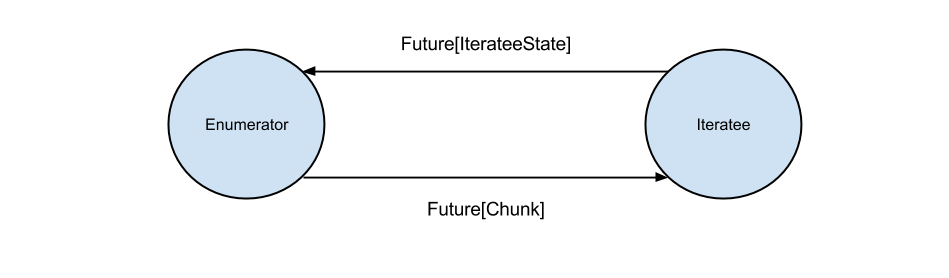
\includegraphics[width=1.0\textwidth]{img/itenum.png}}
    \caption{Back-pressure mechanism with Enumerator and Iteratee using Futures}
    \label{fig:itenum}
  \end{center}
\end{figure}

Thus we have asynchronous production and consumption with the consumer that "tells" (via its future state) to the producer that it is ready to 
consume more chunks (or not). This mechanism in known as \verb|back-pressure| and allows the consumer to slow down the producer rate depending on its 
own processing speed. 

With back-pressure, we can differentiate two kinds of producers: \textit{cold} sources and \textit{hot} sources. Cold sources are sources that
produces chunks from a static durable collection, meaning that the consumer can process the stream at his own speed without the risk of losing events.
On the contrary, \textit{hot} sources are for example events coming from a network connection. If the consumer is not ready to consume the next chunk,
a choice has to be done (drop the event, buffer it, ...). These problems will be dealt with more specifically further in the report.
\\

Futures and Iteratees compositions allows to model the asynchronous processing of both a single value and a stream of values, but 
they are not abstractions to built your entire program on (they are parts of your program).
The Actor model is an abstraction to model your entire application to easily handle concurrency, distribution and fault-tolerance, and can use Futures and Iteratees.

\section{Actor model}

First of all, it should be noted the Actor model is not a purely functional model as it use some side-effects. It is generally said that it sits between functional and
imperative. Nevertheless, we will study it in this part as it integrates very well with functional code and is part of Scala's way of handling concurrency.
The examples use the Akka framework \footfullcite{bib:akka} that provides actor systems for the JVM in Scala.
\\

\subsection{The actor model in Akka}

In imperative languages, synchronization of different concurrent operations is usually done by using locks (including synchronization blocks in Java). 
However, locks is a very low-level primitive that can easily lead to problems like dead-lock, data inconsistency if not enough locks, 
slow performance if too many locks. Moreover, IO is generally done explicitly via sockets.

An actor system is a higher level abstraction to deal with concurrency and synchronization, and abstracts away sockets by providing a location transparent model
via message passing. It enables simple fault-tolerance and distribution.
\\

An actor is a lightweight concurrent entity. Basically, an actor receives messages from other actors and send messages to other actors. Upon the reception of 
a message, it can modify its internal state (actors can be stateful), send messages to other actors, and change its message handling behavior of the next messages.
Each actor has one mailbox that corresponds to a FIFO queue of incoming messages.
It is guaranteed that message processing is sequential inside a same actor, i.e one should not have to worry about concurrency problems inside an actor. Listing
\ref{lst:actorexample} shows how to define a simple Actor that counts the number of messages it receives. Messages can sent to him concurrently without worrying
about synchronization problems.

\begin{listing}[h]
\begin{minted}[fontsize=\codesize, frame=lines, framesep=2mm]{scala}
case object Message

class Counter extends Actor {
  var counter = 0

  def receive = {
    case Message => 
      counter = counter + 1
  }
}

val system = ActorSystem("MySystem")
val counter = system.actorOf(Props[Counter], name = "counter")

// Sending concurrently 100 messages to the actor 
// (the send operation "!" do not block or wait for an ack)
(1 to 100).par foreach (_ => counter ! Message)
\end{minted}
\caption{A counter actor}
\label{lst:actorexample}
\end{listing}

Another important part of the actor model of Akka is the Tree-like hierarchical organization between actors, called Supervision.
A parent that create child actors is responsible for them, meaning that it should handle their possible failures (by stopping them,
restarting them, etc).
\\

Last but not least, the fact that actors communicates only via message passing (share-nothing architecture) allows location transparency, which
enables easy distribution. In Akka, the fact that one or several actors are located on different machines is written in a configuration file, meaning that
one can write the exact same code for a program that execute locally or in a distributed fashion.

Under the hood, a Scheduler is in charge of multiplexing actors into threads, like the ExecutionContext multiplexes Futures into threads.

\subsection{Mixing Actors with Futures}
\label{sec:mixingactorfuture}

Akka's actors can be used with library that use Futures. However, one should pay attention to the mix between SchedulerContext 
and futures' ExeceutionContext. Akka ensures that all message processing are sequential (so that one does not have to worry about concurrency problems inside
an actor), but if the result of a future tries to modify the internal state of an actor, Akka can not ensure the sequentiality as it only control the SchedulerContext
that is used to process incoming messages. To avoid this, one must use the \textit{pipeTo} pattern that transform the result a Future in a message sent to the actor.
Listing \ref{lst:akkasafeunsafe} illustrates this mechanism.

\begin{listing}[h]
\begin{minted}[fontsize=\codesize, frame=lines, framesep=2mm]{scala}
case class Message(data: String)
case class Result(result: String)

// An actor that receive a Message, call an async method to process it,
// store the result of the processing
class ProcessActor extends Actor {
  var storeResults = Seq.empty[String]

  def receive = {
    case Message(data: String) => 
      val futureResult = process(data)
      futureResult map { result =>
        Result(result)
      } pipeTo self

    case Result(result: String) =>
      storeResults = storeResults :+ result
  }
}

// Below is an example that is concurrently unsafe because the future 
// modify the internal state of the actor
class UnsafeActor extends Actor {
  var storeResults = Seq.empty[String]

  def receive = {
    case Message(data: String) => 
      val futureResult = process(data)
      futureResult foreach { result =>
        storeResults = storeResults :+ result
      }
  }
}
\end{minted}
\caption{Mixing Futures with Actors}
\label{lst:akkasafeunsafe}
\end{listing}

The following chapter describes the architecture and implementation of the platform that makes heavy use of the functional programming abstractions which have been 
presented in this chapter.


